%%%%%%%%%%%%%%%%%%%%%%%%%%%%%%%%%%%%%%%%%
% Short Sectioned Assignment LaTeX Template Version 1.0 (5/5/12)
% This template has been downloaded from: http://www.LaTeXTemplates.com
% Original author:  Frits Wenneker (http://www.howtotex.com)
% License: CC BY-NC-SA 3.0 (http://creativecommons.org/licenses/by-nc-sa/3.0/)
%%%%%%%%%%%%%%%%%%%%%%%%%%%%%%%%%%%%%%%%%

%----------------------------------------------------------------------------------------
%	PACKAGES AND OTHER DOCUMENT CONFIGURATIONS
%----------------------------------------------------------------------------------------

\documentclass[paper=a4, fontsize=10pt]{scrartcl} % A4 paper and 11pt font size

% ---- Entrada y salida de texto -----
\usepackage{ marvosym }

\usepackage[T1]{fontenc} % Use 8-bit encoding that has 256 glyphs
\usepackage[utf8]{inputenc}
%\usepackage{fourier} % Use the Adobe Utopia font for the document - comment this line to return to the LaTeX default

% ---- Idioma --------

\usepackage[spanish, es-tabla]{babel} % Selecciona el español para palabras introducidas automáticamente, p.ej. "septiembre" en la fecha y especifica que se use la palabra Tabla en vez de Cuadro

% ---- Otros paquetes ----

\usepackage{url} % ,href} %para incluir URLs e hipervínculos dentro del texto (aunque hay que instalar href)
\usepackage{amsmath,amsfonts,amsthm} % Math packages
%\usepackage{graphics,graphicx, floatrow} %para incluir imágenes y notas en las imágenes
\usepackage{graphics,graphicx, float} %para incluir imágenes y colocarlas

% Para hacer tablas comlejas
%\usepackage{multirow}
%\usepackage{threeparttable}

%\usepackage{sectsty} % Allows customizing section commands
%\allsectionsfont{\centering \normalfont\scshape} % Make all sections centered, the default font and small caps

\usepackage{fancyhdr} % Custom headers and footers
\pagestyle{fancyplain} % Makes all pages in the document conform to the custom headers and footers
\fancyhead{} % No page header - if you want one, create it in the same way as the footers below
\fancyfoot[L]{} % Empty left footer
\fancyfoot[C]{} % Empty center footer
\fancyfoot[R]{\thepage} % Page numbering for right footer
\renewcommand{\headrulewidth}{0pt} % Remove header underlines
\renewcommand{\footrulewidth}{0pt} % Remove footer underlines
\setlength{\headheight}{13.6pt} % Customize the height of the header

\numberwithin{equation}{section} % Number equations within sections (i.e. 1.1, 1.2, 2.1, 2.2 instead of 1, 2, 3, 4)
\numberwithin{figure}{section} % Number figures within sections (i.e. 1.1, 1.2, 2.1, 2.2 instead of 1, 2, 3, 4)
\numberwithin{table}{section} % Number tables within sections (i.e. 1.1, 1.2, 2.1, 2.2 instead of 1, 2, 3, 4)

\setlength\parindent{0pt} % Removes all indentation from paragraphs - comment this line for an assignment with lots of text

\newcommand{\horrule}[1]{\rule{\linewidth}{#1}} % Create horizontal rule command with 1 argument of height

% Añadidos por Rubén Morales Pérez
\usepackage[hidelinks]{hyperref} 
\usepackage[usenames]{color}
\usepackage{verbatim}
\usepackage{listings}
\usepackage{multicol}
\usepackage{caption}
\usepackage{subcaption}

\definecolor{Cyan}{RGB}{0,32,96}
\definecolor{codegreen}{rgb}{0,0.6,0}
\definecolor{codegray}{rgb}{0.5,0.5,0.5}
\definecolor{codepurple}{rgb}{0.58,0,0.82}
\definecolor{backcolour}{rgb}{0.95,0.95,0.92}

\lstdefinestyle{mystyle}{
	backgroundcolor=\color{backcolour},   
	commentstyle=\color{codegreen},
	keywordstyle=\color{magenta},
	numberstyle=\tiny\color{codegray},
	stringstyle=\color{codepurple},
	basicstyle=\footnotesize,
	breakatwhitespace=false,         
	breaklines=true,                 
	captionpos=b,                    
	keepspaces=true,                 
	numbers=left,                    
	numbersep=5pt,                  
	showspaces=false,                
	showstringspaces=false,
	showtabs=false,                  
	tabsize=2
}
\lstset{style=mystyle}



% Paquetes añadidos a la plantilla
\usepackage{anysize}
\marginsize{3cm}{3cm}{2.5cm}{2.5cm}
%\usepackage[scaled]{uarial}
% Para instalar la fuente seguir instrucciones de https://tex.stackexchange.com/questions/60644/latex-error-file-uarial-sty-not-found





%----------------------------------------------------------------------------------------
%	TÍTULO Y DATOS DEL ALUMNO
%----------------------------------------------------------------------------------------

\title{	
\normalfont \normalsize 
\textsc{\textbf{Ingeniería de Servidores (2016-2017)} \\ Grado en Ingeniería Informática \\ Universidad de Granada} \\ [25pt] % Your university, school and/or department name(s)
\horrule{0.5pt} \\[0.4cm] % Thin top horizontal rule
\huge IBM mainframes \\ Watson Machine Learning \\ % The assignment title
\horrule{2pt} \\[0.5cm] % Thick bottom horizontal rule
}

\author{Francisco Javier Morales Piquerasa
	\\ Rubén Morales Pérez} % Nombre y apellidos

\date{\normalsize\today} % Incluye la fecha actual

%----------------------------------------------------------------------------------------
% DOCUMENTO
%----------------------------------------------------------------------------------------

\begin{document}

\maketitle % Muestra el Título
\newpage %inserta un salto de página
\tableofcontents % para generar el índice de contenidos
\listoffigures
\listoftables

\newpage


\section{Resumen}
% Entre 5 y 15 líneas: 


\section{Memoria}
\subsection{Introducción}
Hay varios retos que tienen las compañías actualmente para poder mantenerse competitivas en un mundo cada vez más globalizado.
El mundo de las tecnologías de la información y la comunicación toma un papel fundamental, cada vez hay corporaciones con página web, aplicaciones u ofreciendo información actualizada a través de redes sociales.

\

Una vez que tenemos una base tecnológica es recomendable pasar al siguiente nivel, tener información suficiente y de calidad recopilada de forma que podamos obtener un beneficio competitivo con ella.
Entonces entra en juego el análisis de datos y mantener esa información segura, por temas de protección de datos.
Aquí es donde interviene IBM mainframes \cite{ibm-m}, grandes ordenadores que nos ofrecen computación en la nube de forma que podremos almacenar los datos en dichos servidores con cierta garantía y a la vez dejar a estos ordenadores el procesamiento pesado de datos.

\

El primer ordenador digital de propósito general de IBM fue ASCC (\href{https://www-03.ibm.com/ibm/history/exhibits/markI/markI_intro.html}{Automatic Sequence Controlled Calculator}), se desarrolló junto con la Universidad de Hardvard. Entre los sistemas más modernos hablaremos de \href{https://www-03.ibm.com/systems/z/}{z Systems}.



\begin{figure}[H]
	\centering
	\begin{subfigure}{.5\textwidth}
		\centering
		\href{https://www-03.ibm.com/ibm/history/exhibits/markI/markI_intro.html}{		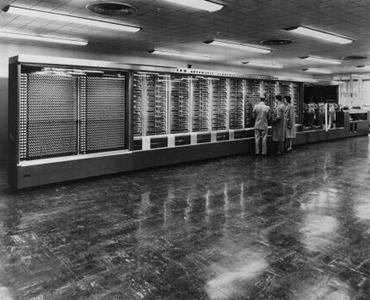
\includegraphics[width=.65\linewidth]{./Imagenes/ascc.jpg}}
		\caption{ASCC}
		\label{fig:ascc}
	\end{subfigure}%
	\begin{subfigure}{.5\textwidth}
		\centering
		\href{https://www-03.ibm.com/systems/z/hardware/z13.html}{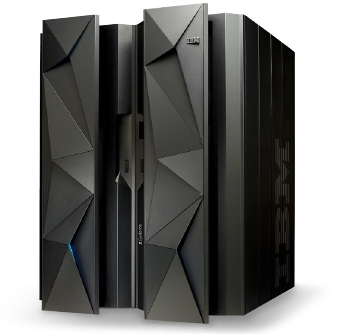
\includegraphics[width=.65\linewidth]{./Imagenes/z13.jpg}}
		\caption{Z13}
		\label{fig:z13}
	\end{subfigure}
\end{figure}



\subsection{Mainframes IBM z Systems}

\subsubsection{Blockchain}





\section{Conclusiones}




%------------------------------------------------
\newpage
\bibliography{citas} %archivo citas.bib que contiene las entradas 
\bibliographystyle{plain} % hay varias formas de citar

\end{document}
